\documentclass[a4paper]{article}
\usepackage[utf8]{inputenc}
\usepackage{indentfirst}
\usepackage{polski}
\usepackage[left=2.5cm,right=2.5cm,top=2cm,bottom=2cm]{geometry}
\usepackage{graphicx}
\linespread{1.3}

\title{\vspace{80mm}Implementacja interfejsu 1wire w VHDL przy użyciu Spartan-3E oraz DS18S20}
\author{Krzysztof Cabała 210047\\ Kinga Wilczek 210063\vspace{110mm}}

\begin{document}
\maketitle
\thispagestyle{empty}

\tableofcontents
\newpage
\listoffigures

\newpage
\section{Wstęp}
Interfejs 1wire jest interfejsem opracowanym przez firmę Dallas Semiconductor do komunikacji między dwoma lub większą liczbą urządzeń przy wykorzystaniu zaledwie jednej lini danych, linii GND (konieczne odniesienie dla poprawnego rozpoznawania stanów logicznych) oraz zasialania gVcc. 
W ramach oszczędności przewodów ogranicza się połączenia do dwóch lini, wtedy układ zasilany jest pasożytniczo z lini danych.
Przykładowe połacznie przedstawia schemat:

\begin{figure}[h]
\begin{center}
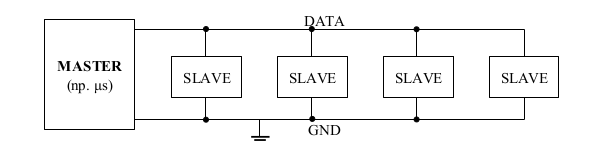
\includegraphics[scale=0.3]{graphics/idea.png}
\end{center}
\label{schemonewire}
\caption{Przykładowe połączenie urządzeń}
\end{figure}

Wyróżnia się urządzania typu Master (najczęsciej mikrokontroler) oraz Slave (peryferia).

\section{Założenia projektowe}
\section{Podstawowe operacje}



\subsection{Inicjalizacja i reset}

Każda próba komunikacji urządzeń master i slave musi zacząć się od sekwencji składającej się z sygnału reset, wysyłanego przez master, po którym następuje sygnał obecności układu slave. Sygnał reset to wymuszony stan 0 trwający przynajmniej 480$\mu$s. Następnie master oczekuje na sygnał obecności innego urządzenia na linii. Następuje wówczas zwolnienie magistrali, co powoduje podciągnięcie jej do stanu wysokiego przez rezystor pull-up. Urządzenie slave wykrywa wówczas narastające zbocze lini i po upływie 15$\mu$s-60$\mu$s sygnalizuje swoją obecność poprzez wymuszenie stanu niskiego na okres 60$\mu$s-240$\mu$s.

\begin{figure}[!h]
\begin{center}
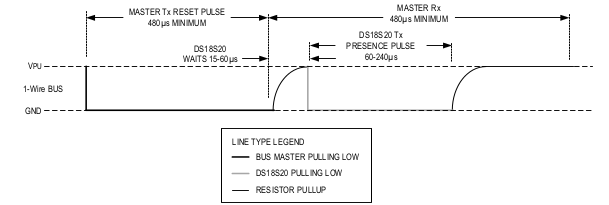
\includegraphics[scale=0.4]{graphics/init.png}
\end{center}
\label{inititming}
\caption{Diagram czasu dla procedury inicjalizacji}
\end{figure}

\subsection{Zapis i odczyt}
\subsubsection{Zapis bitu}
Operacje zapisu bitu realizowane są w ściśle określonych slotach czasowych. Długość jednego slotu wynosić zwykle 60$\mu$s. Próbkowanie dokonywane jest mniej więcej w środku slotu celem uodpornienia na błędy. Pomiędzy kolejnymi operacjami wymagana jest przynajmniej 1$\mu$s odstępu.

Zapis rozpoczyna się wysterowaniem linii danych przez master na poziom niski. Zapis 0 wymaga utrzymania jej w tym stanie przez cały slot. Zapis 1 jest nieco bardziej skomplikowany. Master musi w czasie nie dłuższym niż 15$\mu$s, ale nie krótszym niż 1$\mu$s zwolnić magistralęm tak aby w momencie próbkowania (po 30$\mu$s od zbocza opadającego) była w stanie wysokim. 

\subsubsection{Odczyt bitu}
Odczyt bitu również wymaga 60$\mu$s slotu oraz 1$\mu$s przerwy. Odczyt rozpoczyna się wymuszeniem przez master stanu niskiego na linii danych na czas nie krótszy niż 1$\mu$s i zwolnienie jej (powrót do stanu wysokiego). Po tym sygnale sterowanie linią przejmuje urządzenie slave, wysyłające bit 0 lub 1. Slave po wykryciu zbocza opadającego wymusza stan niski (dla 0) lub utrzymuje  wysoki (dla 1) linii danych. Sygnał musi być wtedy spróbkowany przez master. Przed upłynięciem czasu końca slotu maigistrala zostaje zwolniona przez slave, co powoduje jej powrót do stanu wyokiego.

\begin{figure}[!h]
\begin{center}
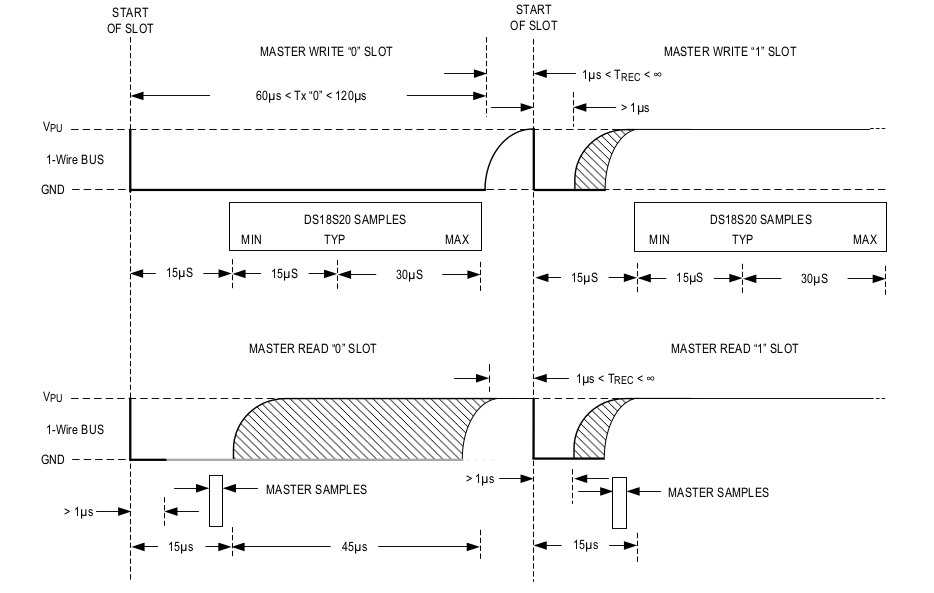
\includegraphics[scale=0.5]{graphics/slots.png}
\end{center}
\label{slotsitming}
\caption{Diagramy czasow dla procedury zapisu i odczytu}
\end{figure}

\section{Implementacja podstawowych operacji}
\section{Transmisja bajtu}
\section{Implementacja transmisji bajtu}
\section{Sekwencja konwersji i odczytu temperatury}
\section{Implementacja konwersji i odczytu temperatury}
\section{Algorytm double dabble}
\section{Implementacja double dabble}
\end{document}